\documentclass[12 pt]{article}
\usepackage[utf8]{inputenc}
\usepackage{fullpage} % use maximum margin
\usepackage{outlines} % add outline
\usepackage{graphicx} % add image

\setlength{\parskip}{1em}  % every new paragraph there's a space

\begin{document}
    
    %title
    \begin{center}
        \Large Chapter 2: Transmission Line
    \end{center}

    \begin{outline}[enumerate]
    \1 Connect what I learned about circuit to electromagnetic theory.
    \1 Kitchoff's voltage and current laws were applied to develop wave equations whose solutions provide an understanding of wave propagation, standing waves, power transfer
    \1 The function of transmission line is to delegate electromagnetic signal
    \1 Transmission line is a two-port network.
      \2 For a dc sourcem there is a generative resistance (R\_g).
      \2 For a ac source, there is a impedance (Z\_g).
      \2 For any thevenin-equivalent circuit, there is always a load (which can be a circuit or a single component)    
    \end{outline}

    \begin{figure}[h!]
        \centering
        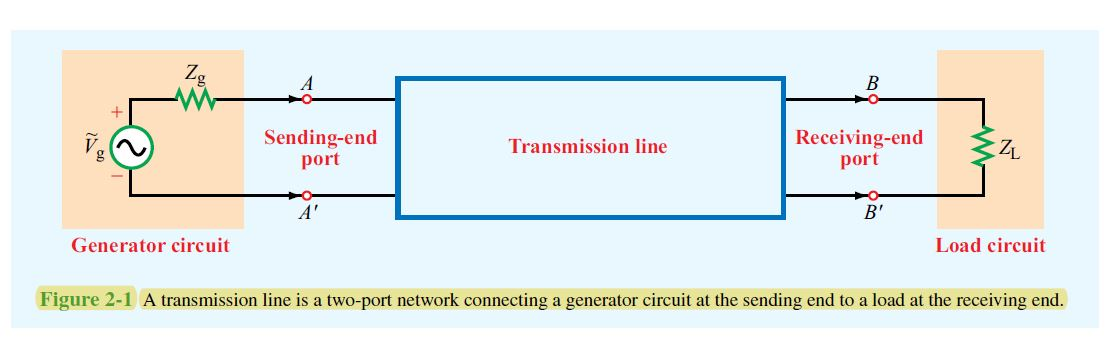
\includegraphics[width=\linewidth]{F2-1.JPG}
        \caption{Transmission line on circuit diagram}
        \label{fig:2-1}
    \end{figure}
    Figure \ref{fig:2-1} shows transmission line.

\end{document}
